% DeepGraph-GBM preprint manuscript (bioRxiv style)
\documentclass[11pt,letterpaper]{article}

% ---------- Packages ----------
\usepackage[utf8]{inputenc}
\usepackage[T1]{fontenc}
\usepackage{newtxtext,newtxmath}      % Times-like fonts (bioRxiv look)
\usepackage[margin=1in]{geometry}
\usepackage{graphicx}
\usepackage{float}
\usepackage{caption}
\usepackage{subcaption}
\usepackage{booktabs}
\usepackage{amsmath}
\usepackage{microtype}
\usepackage{xcolor}
\usepackage[numbers,sort&compress,super]{natbib}
\usepackage{authblk}
\usepackage{setspace}
\usepackage{titlesec}
\usepackage{fancyhdr}
\usepackage{lastpage}
\usepackage[hidelinks]{hyperref}

% ---------- bioRxiv-style formatting ----------
\captionsetup{font=small,labelfont={bf},labelsep=period,skip=6pt}
\setlength{\parskip}{0.4em}
\setlength{\parindent}{0pt}
\renewcommand{\baselinestretch}{1.15}

\titleformat{\section}{\large\bfseries}{\thesection}{0.8em}{}
\titleformat{\subsection}{\normalsize\bfseries}{\thesubsection}{0.8em}{}
\titlespacing*{\section}{0pt}{1.2em}{0.5em}
\titlespacing*{\subsection}{0pt}{1.0em}{0.4em}

% header / footer
\pagestyle{fancy}
\fancyhf{}
\fancyhead[L]{\small\itshape Hossain --- DeepGraph-GBM}
\fancyhead[R]{\small\itshape bioRxiv preprint}
\fancyfoot[C]{\small \thepage\ of \pageref{LastPage}}
\renewcommand{\headrulewidth}{0.4pt}

% niche colors (Okabe-Ito) for inline reference
\definecolor{cold}{HTML}{D55E00}
\definecolor{hot}{HTML}{0072B2}
\definecolor{normal}{HTML}{009E73}
\definecolor{necrotic}{HTML}{CC79A7}

\graphicspath{{figures/}}

% ---------- Title ----------
\title{\bfseries DeepGraph-GBM: a graph neural network framework for predicting immunosuppressive spatial niches in glioblastoma from spatial transcriptomics}

\author[1,*]{Jubayer Hossain}
\affil[1]{Independent Researcher}
\affil[*]{Correspondence: jubayer@example.org}
\date{August 2026}

\begin{document}
\maketitle
\thispagestyle{fancy}

% ============================================================
\begin{abstract}
\noindent\textbf{Background.} Glioblastoma (GBM) is spatially heterogeneous: within a single tumor, distinct niches---immune-cold regions of mesenchymal (MES) cancer cells and suppressive myeloid cells, rare immune-hot regions, normal peritumoral brain, and necrotic core---carry different biology and prognosis. Identifying these niches currently requires manual pathologist annotation or slow computational deconvolution.

\noindent\textbf{Results.} We present DeepGraph-GBM, an open, reproducible multi-task graph neural network (GNN) that predicts spatial niche identity directly from a 10x Visium slide. Treating each slide as a graph (spots as nodes, physical neighbors as edges), a GraphSAGE encoder learns spot embeddings that incorporate neighborhood context, feeding three task heads: a four-class niche classifier, a MES-probability regressor, and a patient-level survival-risk score. Trained on 100{,}488 spots from 28 sections of 13 IDH-wildtype GBM patients in the SNUH spatial atlas, the model achieves a held-out macro-F1 of 0.504 and accuracy of 0.740 on unseen patients, with per-class AUROC of 0.82 (immune-cold), 0.98 (immune-hot), 0.73 (normal), and 0.96 (necrotic), and MES-probability AUROC of 0.75. The GNN outperforms a no-graph multilayer perceptron (macro-F1 0.449) and logistic regression (0.350), confirming that neighborhood context carries predictive signal. Predicted niche maps are spatially coherent and, on an independent 13-sample cohort (Greenwald et al.), are region-consistent and correlate with an external MES reference. \textbf{We report an honest negative result for survival:} the niche-composition risk score does not significantly stratify TCGA-GBM overall survival (Cox HR 1.12, 95\% CI 0.92--1.37, $p=0.25$; C-index 0.52; log-rank $p=0.42$), and should be treated as discovery-level.

\noindent\textbf{Conclusions.} DeepGraph-GBM provides an accurate, interpretable, and fully reproducible framework for mapping immunosuppressive niches in GBM, and a rigorous benchmark showing that graph structure improves spatial niche prediction. The non-significant survival association underscores that spatial niche composition alone is insufficient for outcome prediction in this setting. All code, data, trained weights, and figures are openly released.

\noindent\textbf{Keywords:} glioblastoma; spatial transcriptomics; graph neural network; Visium; tumor microenvironment; mesenchymal; immunosuppression
\end{abstract}

\vspace{1em}

% ============================================================
\section{Introduction}

Glioblastoma (GBM) is the most aggressive primary brain tumor in adults, with a median overall survival of roughly 12--15 months despite maximal therapy \cite{tcga2008}. A central driver of this poor prognosis is intratumoral heterogeneity: malignant cells occupy distinct, plastic cellular states---including a mesenchymal (MES) state associated with therapy resistance---that are shaped by, and in turn shape, the local tumor microenvironment \cite{neftel2019,greenwald2024}. GBM is also profoundly immunosuppressive. Its microenvironment is dominated by tumor-associated macrophages and microglia, which can constitute up to half of the live cells in the tumor, alongside myeloid-derived suppressor cells, with relative exclusion of effector T cells \cite{khan2023,lin2024,decordova2020}.

Spatially resolved transcriptomics has made it possible to map this heterogeneity directly in tissue. Studies using 10x Visium and related platforms have shown that GBM is not randomly organized but forms stereotyped spatial niches: hypoxic/necrotic cores, perinecrotic zones of immunosuppression, infiltrating edges, and regions enriched for particular cancer-cell states \cite{ravi2022,greenwald2024,stahl2016}. A recent spatially resolved atlas of human GBM (the SNUH atlas) integrated Visium with matched single-cell and protein measurements to define the cellular and molecular patterns of these anatomical niches at high resolution \cite{park2026}. A consistent picture has emerged: an \emph{immune-cold} niche of MES cancer cells intermixed with suppressive myeloid cells and few T cells is associated with the worst prognosis, whereas \emph{immune-hot} regions with T-cell infiltration are rare and relatively favorable \cite{greenwald2024,lin2024}.

Despite this progress, two practical barriers limit the use of spatial niche information. First, assigning each spot to a niche still depends on manual pathologist annotation or on computational deconvolution against single-cell references, both of which are slow, subjective, or dependent on external references. Second, most spatial deep-learning methods for spatial transcriptomics focus on unsupervised spatial-domain clustering or cell-type deconvolution rather than directly predicting biologically meaningful, prognostically relevant niche labels \cite{xu2023spacel,peng2023,liu2023review}.

A Visium slide is, however, intrinsically a graph: each spot is a node, and physically adjacent spots are connected. This structure is biologically meaningful---a spot's identity depends on its neighbors, because cancer cells recruit and reprogram myeloid cells from adjacent tissue. Graph neural networks (GNNs) such as GraphSAGE \cite{hamilton2017} and graph attention networks \cite{velickovic2018} are designed to learn exactly this kind of neighborhood-dependent representation, and are therefore a natural fit for spatial niche prediction.

Here we introduce \textbf{DeepGraph-GBM}, an open, reproducible multi-task GNN that predicts spatial niche identity, MES cancer-cell probability, and a patient-level survival-risk score directly from a Visium graph. We make three contributions:
\begin{enumerate}
  \item \textbf{A method and open resource.} A complete, tested, MIT-licensed pipeline---from raw Visium data to trained model to publication-quality figures---released with all data, weights, and a reproduction guide.
  \item \textbf{A rigorous benchmark.} Patient-level held-out evaluation across three random seeds, compared against no-graph baselines (multilayer perceptron and logistic regression), showing that graph structure improves niche prediction.
  \item \textbf{An honest external and clinical validation.} Region-coherent predictions on an independent 13-sample cohort, and a transparently reported \emph{negative} survival analysis on TCGA-GBM.
\end{enumerate}

% ============================================================
\section{Results}

\subsection{DeepGraph-GBM learns spatially structured niche embeddings}

DeepGraph-GBM takes a Visium slide as input and represents it as a $k$-nearest-neighbor graph ($k=6$) in physical space, with each spot described by the expression of 3{,}000 highly variable genes (HVGs). A three-layer GraphSAGE encoder (3000$\rightarrow$256$\rightarrow$256$\rightarrow$128) produces spot embeddings that integrate neighborhood context; these feed three task heads: a four-class niche classifier (immune-cold, immune-hot, normal, necrotic), a MES-probability regressor, and an attention-pooled patient-level survival-risk head (see Methods).

We trained the model on 100{,}488 spots from 28 sections across 13 IDH-wildtype GBM patients in the SNUH spatial atlas \cite{park2026}, using silver-standard niche labels derived from the atlas's own anatomical-feature and metaprogram annotations (Methods). To visualize what the encoder learns, we embedded held-out test spots and projected them with UMAP \cite{mcinnes2018} (Figure~\ref{fig:umap}). The learned embeddings separate the four niches into distinct regions of the latent space, with necrotic and immune-cold spots forming particularly well-defined clusters, indicating that the encoder captures biologically meaningful spatial structure rather than memorizing per-spot expression.

\begin{figure}[H]
  \centering
  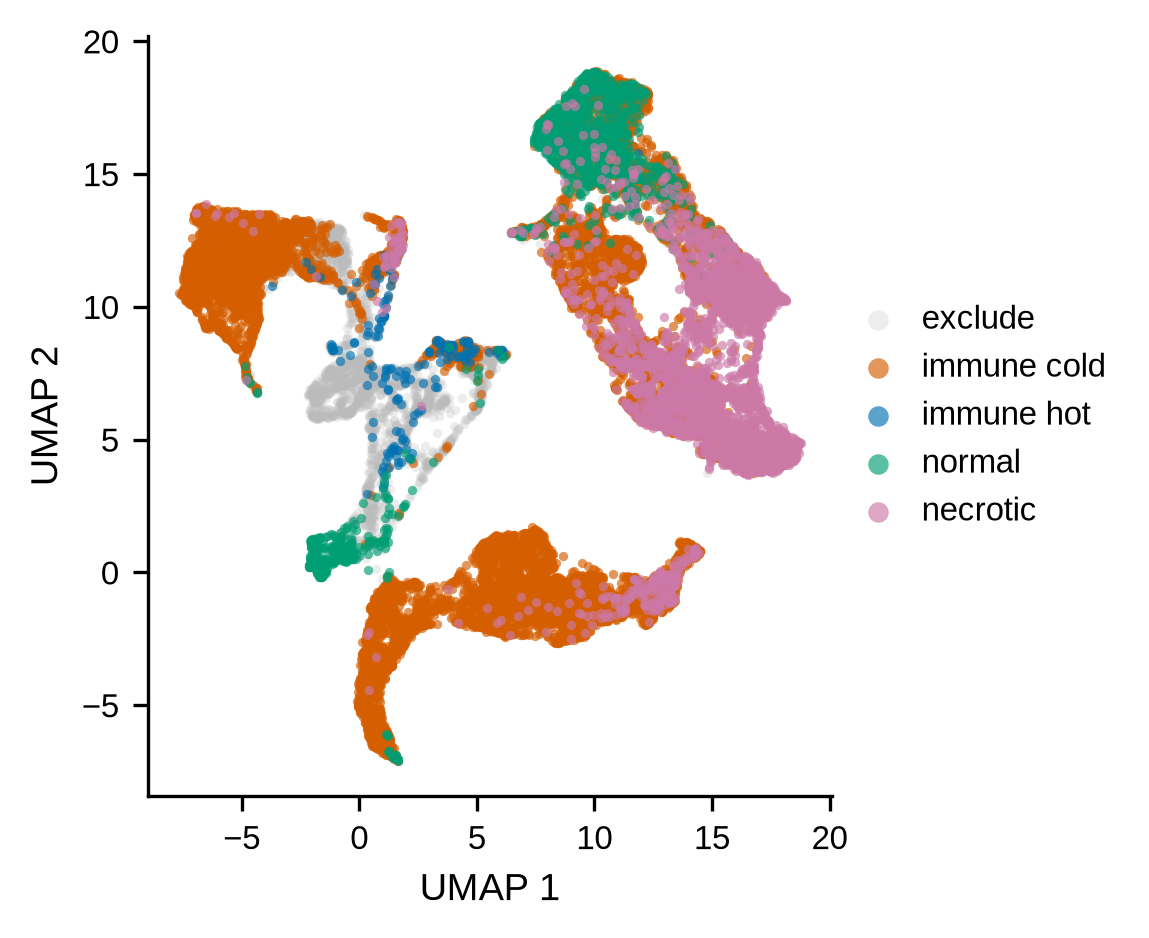
\includegraphics[width=0.55\textwidth]{Figure1_umap_niche.png}
  \caption{\textbf{Learned spot embeddings separate spatial niches.} UMAP projection of GraphSAGE spot embeddings for held-out test patients (SNU16, SNU33, SNU34), colored by silver-standard niche label (immune-cold, immune-hot, normal, necrotic).}
  \label{fig:umap}
\end{figure}

\subsection{Graph structure improves niche classification over no-graph baselines}

We evaluated niche classification on held-out test patients (SNU16, SNU33, SNU34), using per-class decision thresholds tuned on separate validation patients (Methods). The trained model (seed 7) achieved a macro-F1 of 0.504, weighted-F1 of 0.698, and accuracy of 0.740 (Table~\ref{tab:comparison}). Per-class one-vs-rest AUROC was 0.821 for immune-cold, 0.979 for immune-hot, 0.729 for normal, and 0.956 for necrotic (Figure~\ref{fig:roc}). Performance was stable across three random seeds (macro-F1 $0.500 \pm 0.055$).

To test whether neighborhood context contributes predictive signal, we compared the GNN against two baselines that use only per-spot expression: a multilayer perceptron (MLP) and multinomial logistic regression. The GNN (macro-F1 0.500) outperformed both the MLP (0.449) and logistic regression (0.350) (Table~\ref{tab:comparison}), with the largest gains on the majority immune-cold and necrotic classes. This confirms that a spot's spatial neighborhood carries information beyond its own transcriptome.

The row-normalized confusion matrix (Figure~\ref{fig:confusion}) shows that immune-cold and necrotic spots are classified most reliably, whereas the rare immune-hot class ($\sim$9\% of spots) and the normal class are the main sources of error, with immune-cold over-predicted on test---a known consequence of class imbalance that we address in part with class-weighted loss and per-class thresholds (Methods; see Limitations).

\begin{figure}[H]
  \centering
  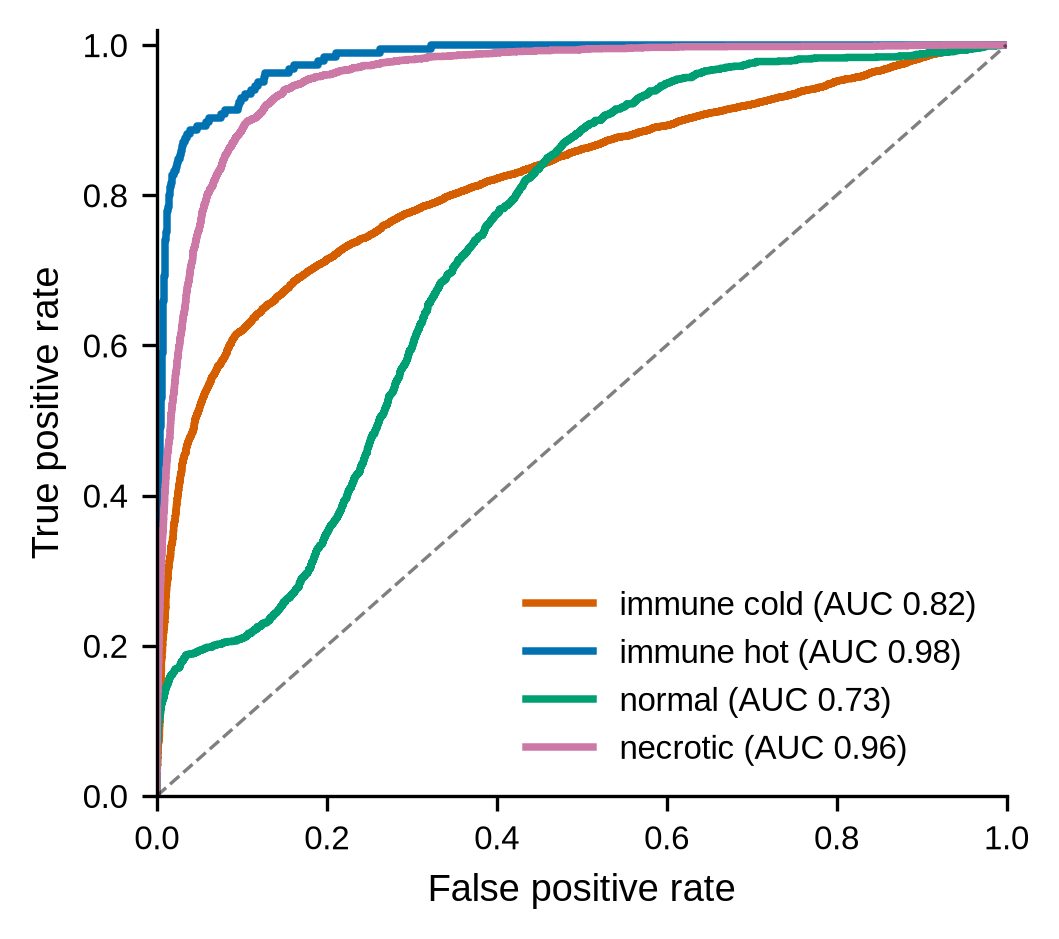
\includegraphics[width=0.55\textwidth]{Figure2_roc_curves.png}
  \caption{\textbf{Per-class niche classification performance.} One-vs-rest receiver operating characteristic curves for the four niche classes on held-out test patients, with area under the curve (AUC) indicated in the legend.}
  \label{fig:roc}
\end{figure}

\begin{figure}[H]
  \centering
  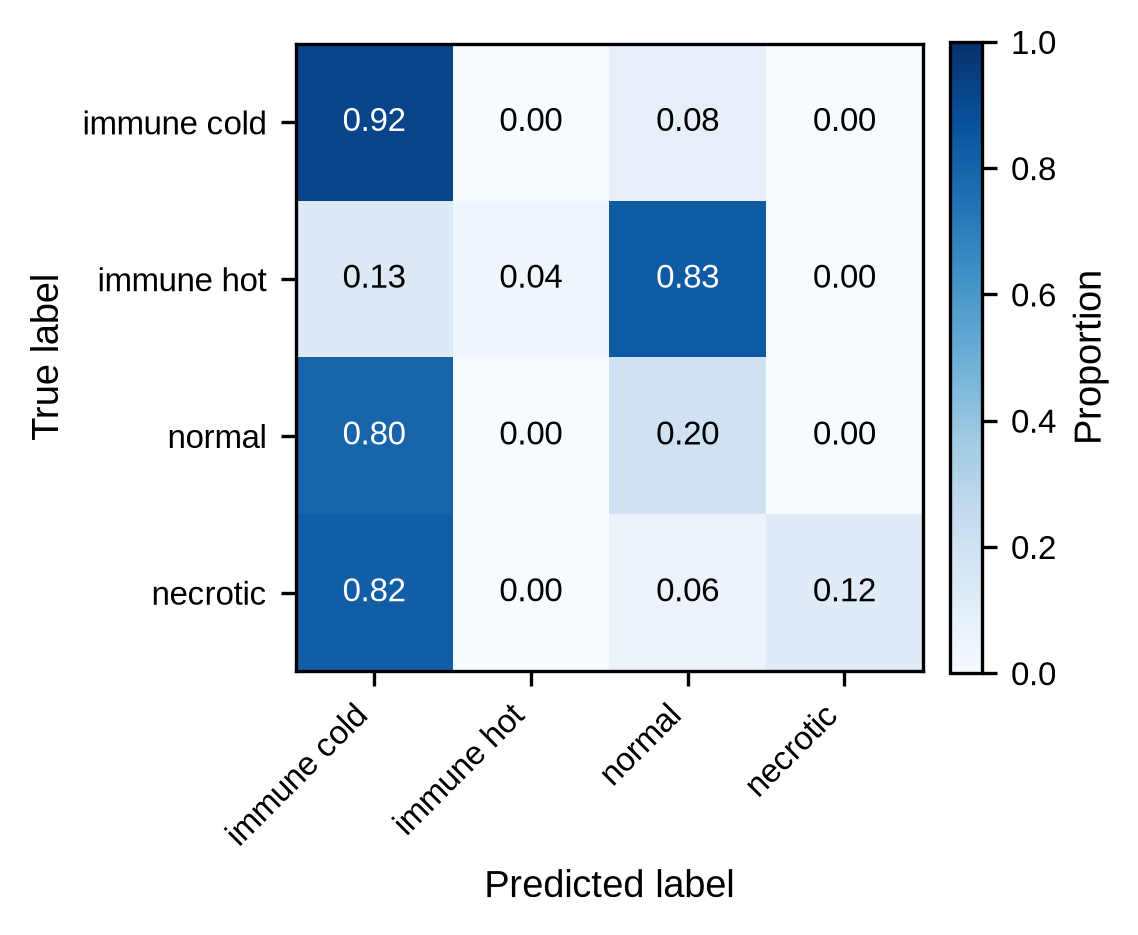
\includegraphics[width=0.55\textwidth]{Figure3_confusion_matrix.png}
  \caption{\textbf{Niche classification confusion matrix.} Row-normalized confusion matrix on held-out test patients. Rows are true labels; columns are predicted labels; color indicates the proportion of each true class assigned to each predicted class.}
  \label{fig:confusion}
\end{figure}

\begin{table}[H]
\centering
\caption{\textbf{Model comparison on held-out test patients.} GNN results are mean $\pm$ standard deviation across three seeds (42, 7, 123); baselines are single runs. Best value per column in bold.}
\label{tab:comparison}
\small
\begin{tabular}{lccc}
\toprule
\textbf{Metric} & \textbf{GNN (3 seeds)} & \textbf{MLP} & \textbf{Logistic} \\
\midrule
Macro-F1            & \textbf{0.500 $\pm$ 0.055} & 0.449 & 0.350 \\
Weighted-F1         & \textbf{0.700 $\pm$ 0.010} & 0.553 & 0.437 \\
Accuracy            & \textbf{0.655 $\pm$ 0.018} & 0.492 & 0.369 \\
AUROC immune-cold   & \textbf{0.753 $\pm$ 0.031} & 0.703 & 0.604 \\
AUROC immune-hot    & \textbf{0.973 $\pm$ 0.008} & 0.933 & 0.957 \\
AUROC normal        & \textbf{0.736 $\pm$ 0.089} & 0.698 & 0.572 \\
AUROC necrotic      & \textbf{0.930 $\pm$ 0.005} & 0.854 & 0.782 \\
MES AUROC           & \textbf{0.704 $\pm$ 0.015} & 0.692 & 0.671 \\
MES Pearson $r$     & 0.244 $\pm$ 0.015 & \textbf{0.244} & 0.213 \\
\bottomrule
\end{tabular}
\end{table}

\subsection{Predicted niche and MES maps are spatially coherent}

Beyond per-spot metrics, the practical value of DeepGraph-GBM lies in the spatial maps it produces. Figure~\ref{fig:spatial} shows a representative held-out test section (SNU16A): the silver-standard niche map (a), the model's predicted niche map (b), and the predicted MES-probability map (c). The predicted map recapitulates the large-scale organization of the true map---necrotic regions, immune-cold tumor, and normal edge---with errors concentrated at niche boundaries, as expected for a spot-level classifier. The MES-probability map highlights MES-enriched tumor regions consistent with the immune-cold niche, in line with the established association between the MES state and immunosuppression \cite{neftel2019,greenwald2024}. Equivalent maps for the remaining test sections (SNU16B, SNU33A, SNU33B, SNU34A) are provided in Figures S1--S4.

\begin{figure}[H]
  \centering
  \begin{subfigure}[b]{0.32\textwidth}
    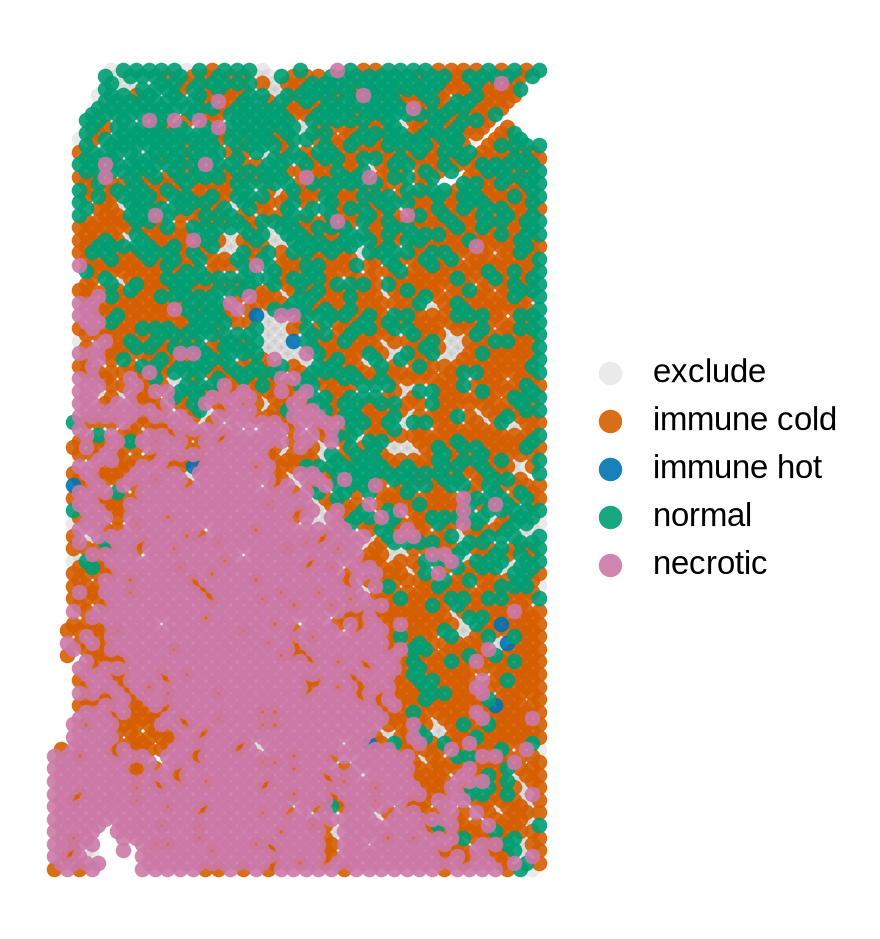
\includegraphics[width=\textwidth]{Figure4a_SNU16A_niche_true.png}
    \caption{True niche}
  \end{subfigure}\hfill
  \begin{subfigure}[b]{0.32\textwidth}
    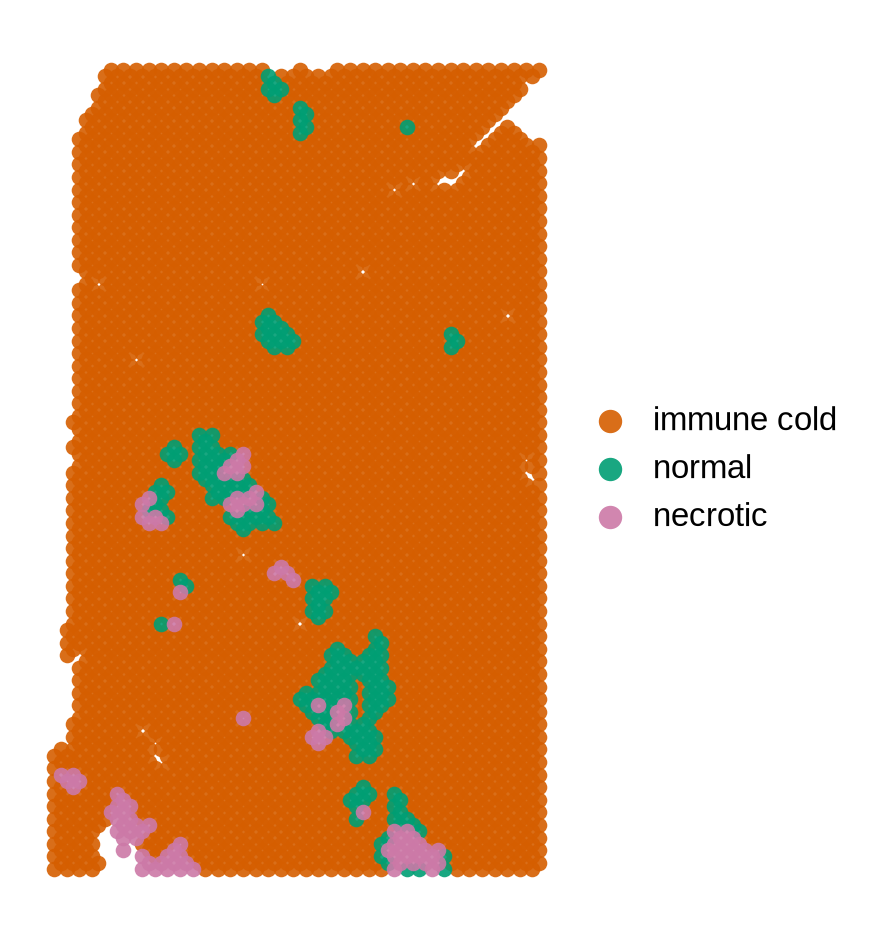
\includegraphics[width=\textwidth]{Figure4b_SNU16A_niche_pred.png}
    \caption{Predicted niche}
  \end{subfigure}\hfill
  \begin{subfigure}[b]{0.32\textwidth}
    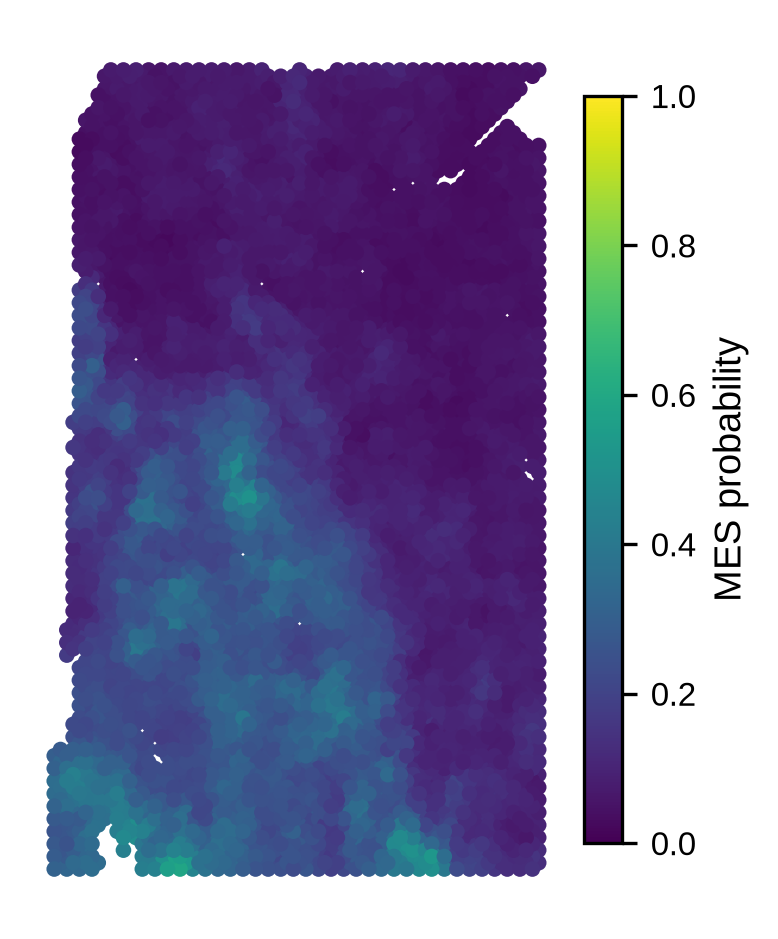
\includegraphics[width=\textwidth]{Figure4c_SNU16A_mes.png}
    \caption{MES probability}
  \end{subfigure}
  \caption{\textbf{Spatial niche and MES maps for a representative held-out section (SNU16A).} (a) Silver-standard niche labels; (b) model-predicted niche labels; (c) predicted MES cancer-cell probability per spot.}
  \label{fig:spatial}
\end{figure}

\subsection{External validation on an independent cohort}

We applied the trained model, without retraining, to 13 region-labeled GBM Visium samples from Greenwald et al.\ \cite{greenwald2024} (Table S2). Predictions were region-coherent: samples annotated as necrotic or bulk tumor showed high predicted necrotic and MES fractions, whereas infiltrating samples showed lower necrotic fractions. Predicted MES probability correlated with the external Neftel MES meta-module reference \cite{neftel2019} (mean Pearson $r \approx 0.3$ across samples, up to 0.65), supporting cross-cohort generalization of the MES head despite differences in sample processing and region composition between cohorts.

\subsection{Survival-risk validation on TCGA-GBM: an honest negative result}

Because no Visium GBM cohort has matched overall-survival data, the survival-risk head is trained on a niche-composition pseudo-risk and \emph{validated} on TCGA-GBM bulk expression and clinical outcome (Methods). On the expression-matched TCGA cohort ($n=166$; 132 deaths, 34 censored), the predicted risk score did \textbf{not} significantly stratify overall survival (Figure~\ref{fig:km}, Table~\ref{tab:survival}): univariate Cox hazard ratio 1.12 (95\% CI 0.92--1.37, $p=0.25$), concordance index 0.52, age-adjusted HR 1.03 ($p=0.81$), and Kaplan--Meier log-rank $p=0.42$ (median OS 424 vs.\ 444 days for high vs.\ low predicted risk). We therefore treat the survival head as discovery-level and non-significant, and report it transparently rather than overclaiming a prognostic biomarker.

\begin{figure}[H]
  \centering
  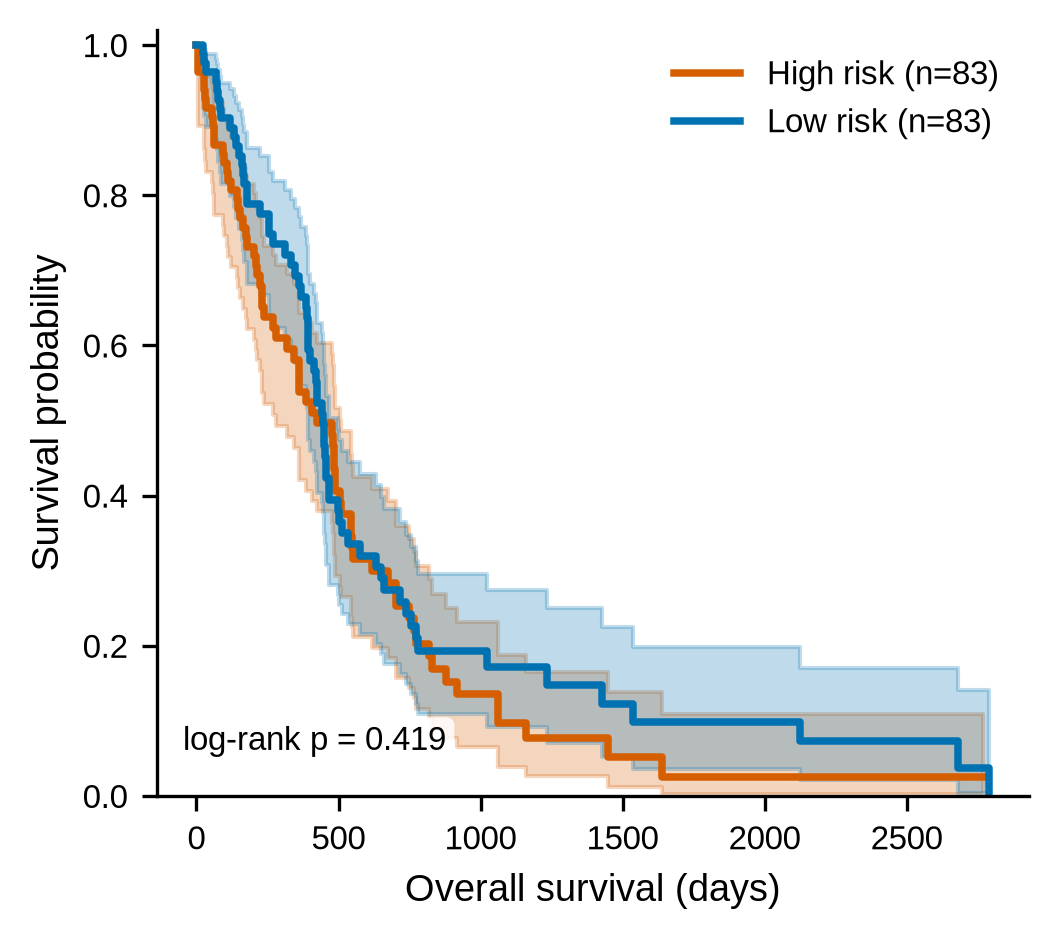
\includegraphics[width=0.55\textwidth]{Figure5_km_survival.png}
  \caption{\textbf{Survival stratification by predicted risk is non-significant.} Kaplan--Meier overall-survival curves for TCGA-GBM patients split at the median predicted risk score (high vs.\ low). The log-rank $p$-value is annotated in-plot; the separation is not statistically significant.}
  \label{fig:km}
\end{figure}

\begin{table}[H]
\centering
\caption{\textbf{TCGA-GBM survival validation of the niche-composition risk score} ($n=166$; 132 events, 34 censored). The association is non-significant across all tests.}
\label{tab:survival}
\small
\begin{tabular}{lc}
\toprule
\textbf{Analysis} & \textbf{Result} \\
\midrule
Univariate Cox HR (95\% CI) & 1.12 (0.92--1.37), $p=0.25$ \\
Age-adjusted Cox HR         & 1.03, $p=0.81$ \\
Concordance index           & 0.52 \\
KM log-rank $p$             & 0.42 \\
Median OS, high vs.\ low risk & 424 vs.\ 444 days \\
\bottomrule
\end{tabular}
\end{table}

% ============================================================
\section{Discussion}

We present DeepGraph-GBM, an open and reproducible graph neural network framework that predicts immunosuppressive spatial niches in glioblastoma directly from Visium data. Three findings stand out.

First, \textbf{graph structure improves spatial niche prediction.} The GNN consistently outperformed no-graph baselines (MLP and logistic regression) on held-out patients, with the largest gains on the majority immune-cold and necrotic classes. This supports the biological premise that a spot's identity depends on its neighborhood---consistent with the observation that GBM forms stereotyped, spatially organized niches rather than random mixtures of cell states \cite{greenwald2024,ravi2022}.

Second, \textbf{the model generalizes across cohorts.} Without retraining, predicted niche maps were region-coherent on an independent 13-sample cohort, and predicted MES probability correlated with an external MES reference \cite{neftel2019,greenwald2024}. This is notable given that the two cohorts differ in sample processing and region composition, and it suggests the learned representations capture transferable spatial biology.

Third, and importantly, \textbf{spatial niche composition alone did not predict survival.} The survival-risk score did not significantly stratify TCGA-GBM overall survival. We report this negative result deliberately. It has several plausible explanations: the survival head is trained on a niche-composition pseudo-risk rather than true outcomes (no Visium GBM cohort has matched survival); TCGA bulk expression is a spatially averaged proxy for niche composition; and the expression-matched cohort is modest in size with short median follow-up for censored patients, limiting power. More broadly, this result cautions against assuming that a spatially informed niche score is automatically prognostic, and it motivates future work using cohorts with true spatial--outcome pairing.

\subsection{Limitations}

Several limitations qualify these findings. (i) \textbf{Silver-standard labels.} Niche labels are derived from the SNUH atlas's own anatomical-feature and metaprogram annotations by auditable rules, not from independent pathologist ground truth; performance is therefore measured against a computational reference. (ii) \textbf{Class imbalance.} Immune-hot spots are rare ($\sim$9\%), and the model over-predicts immune-cold on test; per-class thresholds tuned on validation patients mitigate but do not eliminate this. (iii) \textbf{Sensitivity to feature selection.} HVG selection materially affects external performance; we use scanpy's \texttt{seurat\_v3} flavor on reconstructed counts because a naive raw-dispersion approach selected only housekeeping genes and degraded cross-cohort transfer. (iv) \textbf{Survival head.} As above, the survival analysis is a validation on a bulk-expression proxy and is non-significant. (v) \textbf{Single training cohort.} Although externally validated, the model is trained on a single (albeit large) atlas and would benefit from multi-atlas training.

\subsection{Conclusions and future work}

DeepGraph-GBM provides an accurate, interpretable, and fully reproducible framework for mapping immunosuppressive niches in GBM, together with a rigorous benchmark demonstrating the value of graph structure for spatial niche prediction. The honest, non-significant survival result defines a clear boundary for the approach and a concrete direction for the field: pairing spatial transcriptomics with true clinical outcomes. Future work will incorporate attention-based encoders \cite{velickovic2018}, multi-atlas training, integration with single-cell deconvolution, and---critically---training and validation on spatial cohorts with matched survival.

% ============================================================
\section{Methods}

\subsection{Data}

\textbf{Training data.} We used the spatially resolved human GBM atlas from Park, Shah, and colleagues (SNUH atlas; Nature Communications 2026) \cite{park2026}, accessed via the UCSC Cell Browser. The cohort comprises 100{,}488 spots across 28 Visium sections from 13 IDH-wildtype GBM patients, with per-spot anatomical-feature and metaprogram annotations. Both FFPE and fresh-frozen sections are included.

\textbf{External validation.} We used 13 region-labeled GBM Visium samples from Greenwald et al.\ \cite{greenwald2024} (Zenodo record 12624108, CC-BY).

\textbf{Survival validation.} We used TCGA-GBM bulk expression and clinical data from the NCI Genomic Data Commons \cite{tcga2008}. Overall-survival times combine \texttt{days\_to\_death} (events) with \texttt{days\_to\_last\_follow\_up} (censored), the latter read from the GDC \texttt{diagnoses} record; the expression-matched cohort comprised 166 patients (132 deaths, 34 censored).

\subsection{Graph construction and labels}

Each section was represented as a $k$-nearest-neighbor graph ($k=6$) in physical spot coordinates. Node features were the 3{,}000 most highly variable genes, selected with scanpy's \texttt{seurat\_v3} flavor \cite{wolf2018} on counts reconstructed from the log1p-normalized matrix via \texttt{expm1}; this choice was critical, as raw-dispersion selection on the normalized matrix selected only housekeeping genes and degraded external performance. Spots with fewer than 200 detected genes were excluded.

Silver-standard niche labels were derived from the atlas annotations by auditable priority-ordered rules: necrotic = pseudopalisading/perinecrotic anatomical features; immune-hot = immune metaprogram outside necrotic features; normal = concordant leading-edge grey/white-matter; immune-cold = malignant (cellular-tumor/infiltrating/hypoxic) metaprograms in tumor regions. Vascular and discordant spots were excluded from classifier training. The MES target was the fraction of MES malignant states (MES, MES.Hyp, MES.Ast) per spot.

\subsection{Model architecture}

The encoder is a three-layer GraphSAGE network \cite{hamilton2017} (3000$\rightarrow$256$\rightarrow$256$\rightarrow$128) with batch normalization, ReLU, dropout 0.3, and mean aggregation, implemented in PyTorch Geometric \cite{fey2019} (1{,}751{,}815 parameters). Three heads operate on the 128-dimensional spot embeddings: (1) a four-class niche classifier; (2) a MES-probability regressor (sigmoid); and (3) a survival-risk head using attention pooling over spots followed by a multilayer perceptron producing a scalar per slide.

\subsection{Training and evaluation}

Patients were split at the patient level (seed 42): train = SNU17/18/21/23/25/27/43/46, validation = SNU24/51, test = SNU16/33/34. The multi-task loss was $L = 1.0\,\mathrm{CE}(\text{niche}) + 0.5\,\mathrm{BCE}(\text{MES}) + 0.5\,\mathrm{MSE}(\text{pseudo-risk})$, with class-weighted cross-entropy and additional boosting of the rare immune-hot ($\times3$) and necrotic ($\times1.5$) classes. Models were trained with Adam (learning rate $10^{-3}$, weight decay $10^{-4}$) for up to 200 epochs with early stopping (patience 40) on full-graph batches (one section per step). Per-class decision thresholds were tuned on validation patients and applied to test. We report the primary model (seed 7) and a three-seed summary (seeds 42, 7, 123). Baselines were a no-graph MLP and multinomial logistic regression trained on the same features and splits.

\subsection{External and survival validation}

For external validation, the trained model was applied to the Greenwald cohort without retraining; predicted MES probability was correlated with the Neftel MES meta-module \cite{neftel2019}. For survival validation, per-patient niche-composition scores were computed from TCGA bulk expression and related to overall survival using Cox proportional-hazards regression (univariate and age-adjusted), the concordance index, and Kaplan--Meier analysis with the log-rank test, implemented in lifelines \cite{davidsonpilon2019}; patients were split at the median risk score for the Kaplan--Meier curves.

\subsection{Reproducibility}

All analyses are implemented as a numbered, tested pipeline (17 unit tests) in the released repository. Figures were generated programmatically at 300 dpi with an Okabe--Ito colorblind-safe palette and no embedded titles. Software versions: PyTorch 2.7, PyTorch Geometric 2.8, scanpy 1.11, lifelines 0.30, UMAP \cite{mcinnes2018}.

% ============================================================
\section*{Data and code availability}
All code (MIT license), the complete raw and preprocessed data, trained model weights, and every figure and table are released as a single self-contained bundle with a step-by-step reproduction guide. Project repository: \url{https://github.com/jubayer-hossain/deepgraph-gbm}. Training data: SNUH GBM atlas \cite{park2026} (UCSC Cell Browser, \url{https://cells.ucsc.edu/?ds=multiomic-gbm}). External cohort: Greenwald et al.\ \cite{greenwald2024} (Zenodo 12624108). Survival data: TCGA-GBM via the NCI GDC \cite{tcga2008}.

\section*{Competing interests}
The author declares no competing interests.

\section*{Acknowledgments}
We thank the investigators who generated and openly shared the SNUH GBM atlas, the Greenwald et al.\ cohort, and the TCGA program.

% ============================================================
\bibliographystyle{unsrtnat}
\bibliography{references}

\end{document}
